\documentclass[onecolumn, 12pt]{report}
\usepackage{hyperref,mathtools,amssymb}
\usepackage{cite}
\usepackage{graphicx}
\usepackage{xcolor}
\usepackage{subcaption}
\usepackage[margin=0.75in]{geometry}

\title{ERCAP Proposal: rotating bosons via CL with AMReX}
%\subject{Many-Body Quantum Mechanics}
\author{Casey Berger, Don Willcox}
\date{\today}

\newcommand{\cb}[1]{{\color{red} \bf[NOTE: #1]}}
\newcommand{\etal}{{\it et al.}}
\newcommand{\beq}{\begin{equation}}
\newcommand{\eeq}{\end{equation}}
\newcommand{\bea}{\begin{eqnarray}}
\newcommand{\eea}{\end{eqnarray}}

\def\CP{{\mathcal P}}
\def\CC{{\mathcal C}}
\def\CH{{\mathcal H}}
\def\CW{{\mathcal W}}
\def\CO{{\mathcal O}}
\def\CZ{{\mathcal Z}}
\def\CD{{\mathcal D}}
\def\del{{\nabla}}

\newcommand*\dif{\mathop{}\!\mathrm{d}}

\begin{document}
TO DO
\begin{itemize}
	\item Streamline and connect introduction paragraphs (copied from dissertation)
	\item Expand discussion of rotating superfluids in introduction
	\item Add more about AMReX and how that comes in
	\item Add references
	\item More on scaling/justifying resources  
\end{itemize}
\section{Motivation}

Quantum many-body systems are foundational to a wide range of interesting physical topics, from very small scales (the quark-gluon plasma of the early universe) to very large ones (understanding the structure of neutron stars). Advances in theoretical treatment of these systems can aid in the development of novel materials, provide insights into the stability of nuclei, push forward the boundaries of knowledge about the origin of the universe, and more. However, all but the simplest of these systems can be extremely challenging to understand at a detailed level. Very few are accessible using analytical methods, and those which must be calculated computationally frequently have limitations that prevent us from exploring some of the most interesting physics. 

Computational methods have allowed for great advances in understanding of quantum many-body systems. However, limitations still exist. The computational complexity of many quantum problems scales exponentially with the size of the system due to the size of the underlying Hilbert space, meaning that many systems of great interest are still inaccessible due to lack of fast or powerful enough computers. Nuclear structure is one such example; numerical solutions to the many-nucleon Schr\"{o}dinger equation can only be achieved for nuclei with atomic mass number of up to four. With well-controlled approximations and innovative methods, calculations can be done for heavier nuclei -- up to nickel ($A = \mathcal{O}(60)$)~\cite{2016AbInitioNuclearStructureReactions}.
Innovative methods are what drive advancement in many-body quantum mechanics. Exact solutions to the many-body Schr\"{o}dinger equation simply require more computational resources than exist, and so creative and intelligent alternatives must be developed.

Some quantum many-body systems are inaccessible to QMC methods, for varying reasons. One of the largest sets of these systems are those which suffer from the sign problem, also called the complex phase problem. This is part of a larger group in computer science known as NP-hard problems, for which no general solution is expected to exist (although it remains a topic of ongoing research). The sign problem can arise when a system doesn't have the desired behavior: a real, positive-valued weight in the path integral. In this case, the crucial step for QMC approaches -- i.e. treating the weight like a probability distribution from which we can sample values of the fields and the observables -- becomes invalid.

One such system is that of rotating bosonic particles. This behavior appears across a range of physical systems and energy scales, from rotating nuclei to pulsars. It is also a system that has been studied thoroughly in the laboratory, using supercooled atomic gases confined with optical traps and stirred with a magnetic field. These experimental studies have revealed much about the behavior of rotating bosonic systems, including the spontaneous formation of vortices which contain the angular momentum of the system, but these behaviors do not yet have a full theoretical description.

\section{The physical system and the algorithm: complex Langevin and AMReX}
Rotating bosonic systems can be described using the path-integral formulation. The bosonic fields are complex scalar fields, and the addition of a rotational term in the action makes the system irretrievably \cb{wc?} complex. In order to treat this action composed of complex-valued fields, we use a method called complex Langevin (CL). 

The complex Langevin method is a stochastic method for treating field-theoretical models with a complex action. Complex Langevin extends the well-established Langevin method to complex-valued fields, evolving those fields in a fictitious time (called Langevin time), resulting in a set of field values distributed with the appropriate weight $e^{-S}$, from which quantities of interest can be computed via a simple statistical average. This treatment has been shown to be successful in toy models for finite quark density QCD~\cite{BergerCLReview} as well as low energy atomic systems such as the polarized unitary Fermi gas~\cite{BergerCLReview}. 

The complex Langevin method complexifies the fields, $\phi$, and evolves the complexified components of the fields according to a set of coupled stochastic differential equations, which include a drift function derived from the action of the system and a gaussian-distributed noise term to satisfy the stochastic properties. From these complexified field components, quantities of interest ("observables") can be calculated and saved. The algorithm for a numerical study of rotating bosons with CL is shown in Fig.~\ref{Fig:Algorithm}.
%
\vspace{-3mm}
\begin{figure}[h]
\centering
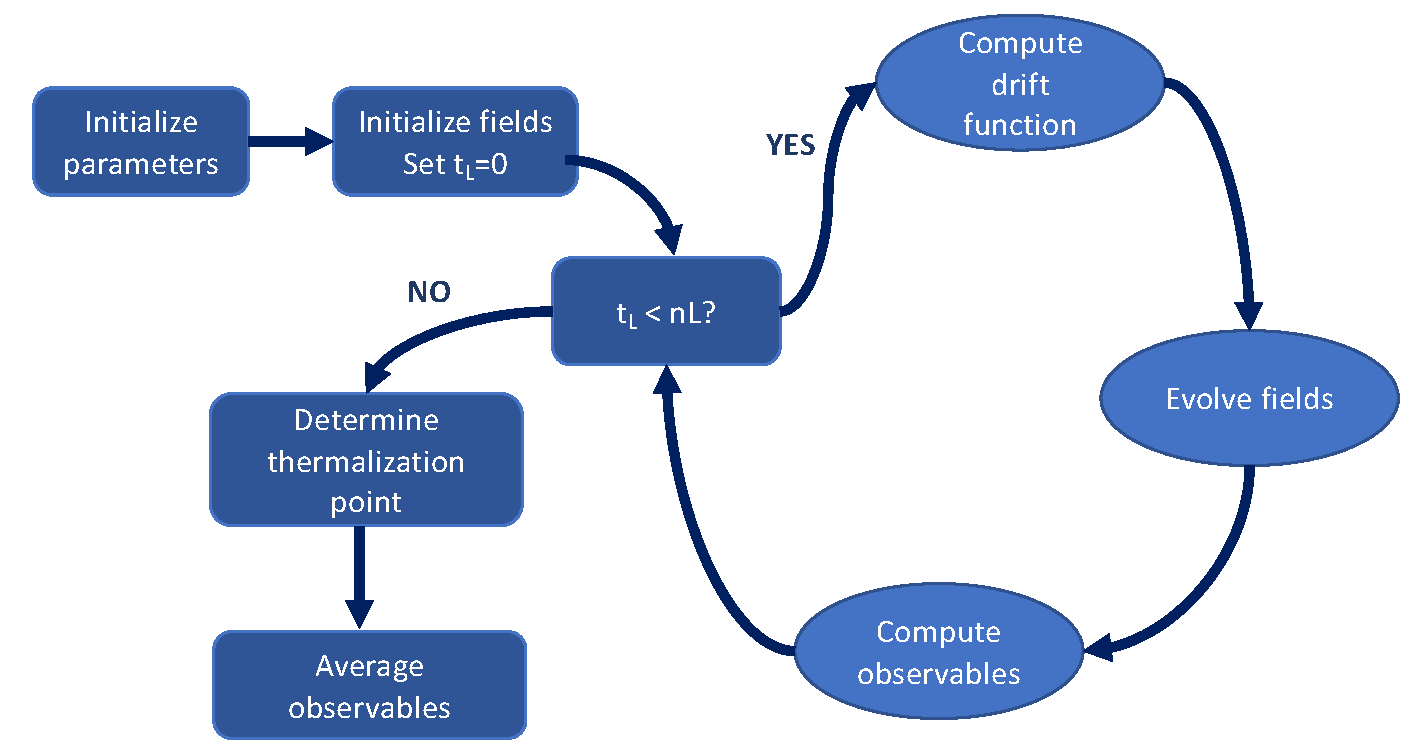
\includegraphics[width=0.6\textwidth]{./algorithm.pdf}
\caption{\label{Fig:Algorithm} Flow chart of the complex Langevin algorithm for the nonlinear sigma model.\vspace{-3mm}}
\end{figure}
\vspace{-3mm}
%

\section{Computational Requirements}

\end{document}